%versi 2 (8-10-2016)
\chapter{Landasan Teori}
\label{chap:teori}

Bab ini membahas tentang landasan teori yang akan digunakan dalam skripsi ini yang diambil dari dua sumber, yaitu ''CodeIgniter Documentation'' karya British Columbia Institute of Technology ~\cite{bcit:17:cidoc} dan ''Sharif Judge Documentation'' karya Mohammad Javad Naderi ~\cite{mjnaderi:14:sharifjudgedoc}.

\section{\textit{CodeIgniter}}
\label{sec:codeigniter} 
 
\textit{CodeIgniter} merupakan sebuah \textit{framework} bagi pengguna yang ingin membangun aplikasi web menggunakan PHP. Tujuan utamanya adalah memungkinkan para pengguna mengembangkan proyek-proyek menjadi lebih cepat dibandingkan menulis kode dari awal. \textit{Framework} ini memiliki banyak libary untuk tugas-tugas yang biasa diperlukan, serta antarmuka dan struktur logis yang sederhana untuk mengakses library ini. CodeIgniter membuat para pengguna lebih fokus pada proyek dengan meminimalkan jumlah kode yang dibutuhkan untuk tugas yanf diberikan~\cite{bcit:17:cidoc}. \\

Beberapa keunggulan dari \textit{CodeIgniter} yaitu:
\begin{itemize}
	\item \textit{Framework} yang Ringan \\
		Inti dari sistem CodeIgniter hanya membutuhkan \textit{library} yang kecil. Hal ini sangat berbeda dengan framework lain yang membutuhkan \textit{resource} yang lebih. \textit{Library} tambahan dimuat secara dinamis atau sesuai dengan permintaan sehingga sistem dapat berjalan cepat.
	\item Menggunakan Konsep M-V-C \\
		\textit{CodeIgniter} menggunakan pendekatan \textit{Model-View-Controller} yang memungkinkan pemisahan anatara logika dan presentasi.
	\item Menghasilkan \textit{Clean URLs} \\
		\textit{URL} yang dihasilkan oleh  \textit{CodeIgniter} berish dan \textit{search-engine friendly}. \textit{CodeIgniter} menggunakan pendekatan \textit{segment-based} seperti: \\example.com/news/article/345
	\item \textit{Packs a Punch} \\
		\textit{CodeIgniter} dilengkapi dengan \textit{library} yang umumnya diperlukan untuk tugas pengembangan web seperti mengakses database, mengirim email, memvalidasi data \textit{form}, menjaga \textit{session}, memanipulasi gambar, bekerja dengan \textit{XML-RPC} data dan masih banyak lagi.
	\item \textit{Extensible} \\
		Sistem dapat dengan mudah diperluas dengan menggunakan \textit{library} pengguna, \textit{helper}, atau melalui \textit{class extensions} dan \textit{system hooks}.
	\item Tidak Membutuhkan \textit{Template Engine} \\
		\textit{CodeIgniter} dilengkapi dengan \textit{template parser} sederhana yang dapat digunakan secara opsional. \textit{Template Engine} tidak dapat menandingi kinerja dari \textit{native} PHP. Sintak yang harus dipelajari untuk menggunakan \textit{Template Engine} biasanya lebih mudah dari mempelajari dasar-dasar PHP. Perhatikan potongan kode PHP di bawah ini: \\
		\begin{lstlisting}[backgroundcolor = \color{lightgray}]
<ul>
<?php foreach ($addressbook as $name):?>
<li><?=$name?></li>
<?php endforeach; ?>
</ul>
	\end{lstlisting}
		
		Sangat berlawanan dengan \textit{pseudo-code} yang digunakan oleh \textit{Template Engine}: \\
	\begin{lstlisting}[backgroundcolor = \color{lightgray}]
<ul>
{foreach from=$addressbook item="name"}
<li>{$name}</li>
{/foreach}
</ul>
		\end{lstlisting}
		Terlihat \textit{Template Engine} sedikit lebih bersih, namun harus ditukar dengan performa yang kurang baik karena \textit{pseudo-code} harus dikonversi kembali menjadi PHP. Salah satu tujuan dari \textit{CodeIgniter} adalah performa maksimal, oleh karena itu \textit{CodeIgniter} tidak menggunakan \textit{Template Engine}.
	\item Dokumentasi yang Baik \\
		Dokumentasi merupakan salah satu bagian terpenting dari kode itu sendiri. \textit{CodeIgniter} berkomitmen membuat kode yang sangat bersih dan terdokumentasi dengan baik. 
\end{itemize}

\subsection{Fitur-fitur CodeIgniter}
Berikut beberapa fitur utama yang terdapat pada \textit{framework CodeIgniter} seperti:
\begin{itemize}
	\item Sistem berbasis \textit{MVC}
	\item \textit{Framework} yang ringan
	\item \textit{Database Class} yang lengkap dengan dukungan untuk beberapa platform
	\item Dukungan \textit{query builder} untuk database
	\item \textit{Form} dan validasi data
	\item Keamanan dan \textit{XSS Filtering}
	\item \textit{Session Management}
	\item \textit{Email Sending Class}
	\item \textit{Image Manipulation Library}
	\item \textit{File Uploading Class} 
	\item \textit{Calendaring Class}
	\item \textit{Unit Testing Class}
\end{itemize}

\subsection{\textit{Flow Chart} Aplikasi}
Gambar~\ref{fig:flow} menunjukan bagaimana data mengalir ke seluruh sistem~\cite{bcit:17:cidoc}:
\begin{figure}[H]
	\centering  
	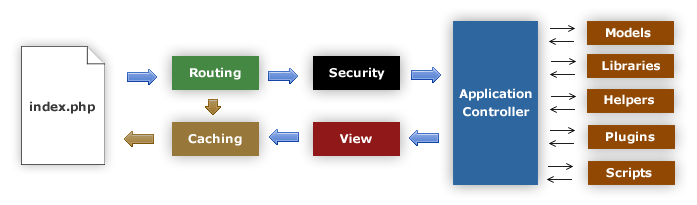
\includegraphics[scale=1]{appflowchart}  
	\caption[\textit{Flow Chart} Aplikasi]{\textit{Flow Chart} Aplikasi} 
	\label{fig:flow} 
\end{figure} 

\begin{enumerate}
	\item File \textit{index.php} berfungsi sebagai \textit{front controller} dan menginisialisasi \textit{resource} utama yang dibutuhkan untuk menjalankan \textit{CodeIgniter}.
	\item \textit{Router} memeriksa \textit{HTTP request} untuk menentukan apa yang harus dilakukan.
	\item Jika terdapat \textit{file cache}, maka akan langsung dikirimkan ke \textit{browser}.
	\item \textit{HTTP request} dan data pengguna yang dikirim akan terlebih dahulu disaring untuk alasan keamanan. \textit{Application controller} akan dimuat setelah proses penyaringan selesai.
	\item \textit{Controller} akan memuat \textit{model, core libraries, helpers} dan \textit{resource} lain yang dibutuhkan untuk memproses permintaan khusus.
	\item \textit{View} akan di \textit{render} kemudian dikirim ke web \textit{browser}. Jika proses \textit{caching} diaktifkan, maka \textit{View} akan di \textit{cache} terlebih dahulu sehingga permintaan berikutnya dapat dilayani.
\end{enumerate}

\subsection{\textit{Model-View-Controller}}
\textit{CodeIgniter} merupakan \textit{framework} yang menggunaakan pola pengembangan \textit{Model-View-Controller}. \textit{MVC} adalah pendekatan perangkat lunak yang memisahkan logika aplikasi dari presentasi. Hal tersebut memungkinkan halaman web pengguna memiliki \textit{scripting} yang minimal karena presentasi terpisah dari \textit{scripting} PHP~\cite{bcit:17:cidoc}. \\

	\subsubsection{\textit{Model}}
	\textit{Model} merepresentasikan bagian struktur data pengguna. Biasanya kelas \textit{Model} akan berisikan fungsi-fungsi yang membantu pengguna untuk mengambil, menyimpan, dan memperbarui informasi pada database. Berikut beberapa hal penting yang terdapat pada Model:
	\begin{itemize}
		\item Susunan dari Model \\
		Kelas model berada di direktori application/models/. Model dapat dikelompokkan di dalam sub direktori bila model jika pengguna menginginkannya. Bentuk dasar kode pada kelas model digambarkan seperti berikut ini:
		\begin{lstlisting}[backgroundcolor = \color{lightgray}]
class Model_name extends CI_Model {
	public function_construct()
	{
		parent::_construct();
		//constructor code
	}
}
		\end{lstlisting}
		
		Model\_name adalah nama kelas dari kelas model yang pengguna buat. Penamaan kelas harus dimulai dengan huruf kapital. Pastikan kelas model merupakan turunan dari base Model (class CI\_Model atau MY\_Model).
		
		\item Menghubungkan Sebuah Model \\
		Pada dasarnya model akan dimuat dan dipanggil dari method atau fungsi yang ada pada controller. Untuk menghubungkan model, pengguna harus menggunakan method berikut:
		\begin{lstlisting}[backgroundcolor = \color{lightgray}]
$this->model->model('model_name');
		\end{lstlisting}
		
		Jika model yang pengguna buat terletak di dalam sebuah sub-direktori, maka pengguna harus menyertakan alamat relatif (relative path) dari model yang dibuat. Sebagai contoh, jika model yang pengguna miliki berlokasi di application/models/blog/Queries.php pengguna dapat menghubungkannya dengan cara:
		\begin{lstlisting}[backgroundcolor = \color{lightgray}]
$this->load->model('blog/queries');
		\end{lstlisting}
		
		Pengguna dapat mengakses method yang terdapat pada model menggunakan sebuah objek dengan nama yang sama dengan nama kelas yang pengguna buat sebelumnya:
		\begin{lstlisting}[backgroundcolor = \color{lightgray}]
$this->load->model('model_name');
		
$this->model_name->method();
		\end{lstlisting}
		
		Jika pengguna ingin menggunakan objek yang berbeda untuk sebuah model, maka pengguna dapat menggunakan penamaan (alias) di parameter kedua:
		\begin{lstlisting}[backgroundcolor = \color{lightgray}]
$this->load->model('model_name', 'foobar');
	
$this->foobar->method();
		\end{lstlisting}
		
		Berikut merupakan contoh sebuah controller yang terhubung dengan sebuah model dan menampilkan data hasil olahan model ke view:
		\begin{lstlisting}[backgroundcolor = \color{lightgray}]
class Blog_controller extends CI_Controller {
			
	public function blog()
	{
		$this->load->model('blog');
		
		$data['query'] = $this->blog->data_sepuluh
		_artikel_terakhir();
		
		$this->load->view('blog', $data);
	}
}
		\end{lstlisting}
		
		\item Auto-loading Model \\
		Auto-loading (menghubungkan secara otomatis) model tertentu secara global dapat pengguna lakukan dengan menggunakan pengaturan yang ada pada berkas application/config/autoload.php. Tambahkan model yang ingin pengguna hubungkan secara otomatis selama sistem berjalan: 
		\$autoload['model'] = array('model\_name');
		
		\item Koneksi ke Database \\
		Ketika sebuah model dipanggail, model tidak akan terhubung ke database secara otomatis. Beberapa opsi yang dapat digunakan untuk menghubungkan model ke database:
		\begin{itemize}
			\item Pengguna dapat menghubungkan dengan menggunakan standar metode database antara class Controller atau class Model. \\
			\item Pengguna dapat mengatur sebuah model melakukan \textit{auto-connect} dengan menambahkan nilai \textit{TRUE} (boolean) di parameter ketiga atau mengatur konektivitas sebagaimana yang telah didefinisikan di dalam berkas application/config/database.php:
			\begin{lstlisting}[backgroundcolor = \color{lightgray}]
\$this->load->model('model_name', '', TRUE);
			\end{lstlisting}
			\item pengguna dapat mengatur koneksi secara manual dengan menambahkan \textit{item-item} berupa \textit{array} pada \textit{parameter} ketiga seperti contoh berikut:
			\begin{lstlisting}[backgroundcolor = \color{lightgray}]
$config['hostname'] = 'localhost';
$config['username'] = 'username';
$config['password'] = 'katasandi';
$config['database'] = 'database_name';
$config['dbdriver'] = 'mysqli';
$config['dbprefix'] = '';
$config['pconnect'] = FALSE;
$config['db_debug'] = TRUE;
			
$this->load->model('model_name', '', $config);
			\end{lstlisting}
		\end{itemize}
	\end{itemize}
	
	\subsubsection{\textit{View}}
	\textit{View} merupakan informasi yang akan ditampilkan kepada pengguna. Umumnya \textit{View} merupakan sebuah halaman web, namun pada \textit{CodeIgniter}, \textit{View} dapat berupa bagian-bagian halaman seperti \textit{header} atau \textit{footer}. Selain itu \textit{View} juga dapat berupa halaman \textit{RSS} atau jenis "halaman" lainnya. \textit{View} tidak pernah dipanggil secara langsung, melainkan harus melalui controller karena dalam framework MVC controller berfungsi sebagai pengatur. Untuk memuat tampilan tertentu, pengguna dapat menggunakan \textit{method} berikut:
	\begin{lstlisting}[backgroundcolor = \color{lightgray}]
$this->load->view('name');
	\end{lstlisting}
	
	CodeIgniter dapat menangani beberapa panggilan method \textit{\$this->load->view()} dari dalam controller. Jika lebih dari satu panggilan terjadi, maka panggilan tersebut ditambahkan bersama. Contohnya pengguna ingin memiliki header view, menu view, content view dan footer view. Kode program yang digunakan seperti ini:
	\begin{lstlisting}[backgroundcolor = \color{lightgray}]
class Page{
	public function INDEX(){
		$data['page_title'] = 'Your title';
		$load->view('header');
		$load->view('menu');
		$load->view('content', $data);
		$load->view('footer');
	}
}
	\end{lstlisting}
	
	\subsubsection{\textit{Controller}}
	\textit{Controller} berfungsi sebagai perantara antara \textit{Model}, \textit{View}, dan \textit{resource} lain yang dibutuhkan untuk memproses \textit{HTTP request} dan menghasilkan halaman web. Controller merupakan sebuah kelas yang dinamakan demikian agar dapat dikaitkan dengan URI. Sebagai contoh URI "example.com/index.php/blog/", CodeIgniter akan mencari controller bernama Blog.php dan menjalankannya. Nama controller harus diawali dengan huruf kapital. Selain itu controller juga harus extend kelas "CI\_Controller".
	Perhatikan contoh berikut:
	Contoh yang benar :
\begin{lstlisting}[backgroundcolor = \color{lightgray}]
<?php
class Blog extends CI_Controller {

}
\end{lstlisting}
	
	Contoh yang salah :
\begin{lstlisting}[backgroundcolor = \color{lightgray}]
<?php
class blog extends CI_Controller {

}
\end{lstlisting} 

	Berikut beberapa hal penting yang terdapat pada Controller:
	\begin{itemize}
		\item Method \\
		Untuk menjalankan suatu method, pengembang perlu menuliskannya pada segmen kedua URI. Contoh "example.com/index.php/blog/comments" maka method comments() akan dijalankan pada controller blog.php. Method index() akan dijalankan jika bagian kedua URI kosong. Jika URI mengandung lebih dari dua segment, maka segment-segment tersebut akan dimasukan ke dalam method sebagai parameter.
		
		\item Default Controller \\
		CodeIgniter dapat diperintahkan untuk menjalankan \textit{default controller} jika tidak terdapat URI. Hal ini umumnya terjadi ketika  terdapat permintaan menggunakan URL dasar \textit{website}. Penentuan \textit{default controller} terdapat pada \textit{file} "application/config/routes.php". Perhatikan contoh berikut:
		\begin{lstlisting}[backgroundcolor = \color{lightgray}]
$route['default_controller'] = 'blog';
		}
		\end{lstlisting} 
		Blog merupakan nama kelas controller yang ingin digunakan. Jika pengguna mengakses file index.php utama tanpa menentukan segmen URI, maka akan dijalankan controller blog.
		
		\item Processing Output \\
		CodeIgniter memiliki kelas \textit{output} yang menangani pengiriman data ke \textit{web browser} secara otomatis. Dalam beberapa kasus saat pengguna ingin mengubah cara pengiriman data tersebut, CodeIgniter akan menambahkan method bernama "\_output()" ke \textit{controller} terkait. Jika controller memiliki method bernama "\_output()" maka controller tersebut akan selalu dipanggil oleh kelas "output".
		Contoh penggunaan method "\_output()" : 
		\begin{lstlisting}[backgroundcolor = \color{lightgray}]
public function _output(\$output)
{
	echo $output;
}
		\end{lstlisting}
		
		\item Private Method
		Method-method dengan tipe \textit{private} tidak dapat diakses oleh publik. Method ini hanya dapat diakses oleh method lain dalam \textit{controller} yang sama dan method ini juga tidak dapat diakses melalui URL. Contoh penulisan \textit{private method}:
		\begin{lstlisting}[backgroundcolor = \color{lightgray}]
private function _utility()
{
	// kode program
}
		\end{lstlisting}
		
		Method di atas tidak dapat diakses dengan cara pemanggilan method pada umum seperti berikut:
		\begin{lstlisting}[backgroundcolor = \color{lightgray}]
example.com/index.php/blog/_utility/
		\end{lstlisting}
		
		\item Mengorganisir Controller ke Dalam Sub Direktori \\
		CodeIgniter mengizinkan pengguna untuk mengorganisir \textit{controller} ke dalam sub direktori. Pengguna dapat membuat sub direktori di dalam direktori \textit{application/controllers/} dan simpan kelas \textit{controller} ke dalamnya. Ketika menggunakan fitur ini, pengguna harus menspesifikasikan folder tersebut ke dalam URI. Perhatikan contoh berikut:
		Sebuah controller berlokasi pada direktori
		\begin{lstlisting}[backgroundcolor = \color{lightgray}]
application/controllers/products/Shoes.php
		\end{lstlisting}
		Untuk memanggil controller di atas, URI pengguna akan terlihat seperti ini:
		\begin{lstlisting}[backgroundcolor = \color{lightgray}]
example.com/index.php/products/shoes/show/123
		\end{lstlisting}
	\end{itemize}

\textit{CodeIgniter} memiliki pendekatan yang cukup fleksibel terhadap \textit{MVC} karena \textit{Model} tidak selalu diperlukan. Para pengguna dapat membangun aplikasi minimal  menggunakan \textit{Controller} dan \textit{View}. Hal tersebut dapat dilakukan jika pengguna tidak memerlukan adanya pemisahan tambahan atau pengguna merasa bahwa mempertahankan sebuah \textit{Model} membutuhkan kompleksitas yang lebih tinggi~\cite{bcit:17:cidoc}. 

\subsection{Desain dan Tujuan Arsitektur}
Dari sudut pandang teknis, dan arsitektural, CodeIgniter dibuat dengan tujuan sebagai berikut:
\begin{itemize}
	\item \textit{Dynamic Instation} \\
	Dalam \textit{CodeIgniter}, komponen dimuat dan rutinitas dieksekusi hanya jika diminta. Tidak ada asumsi yang dibuat oleh sistem tentang apa yang mungkin diperlukan di luar resource utama, sehingga sistem ini sangat ringan secara \textit{default}. \textit{Event}, \textit{Controller} dan \textit{View} yang pengguna rancang akan menentukan apa yang dipanggil.
	\item \textit{Loose Coupling} \\
	\textit{Coupling} adalah sejauh mana komponen-komponen dari sistem saling mengandalkan satu sama lain. Semakin sedikit komponen yang bergantung satu sama lain, maka komponen tersebut lebih dapat digunakan kembali dan sistem menjadi fleksibel. Tujuan dari \textit{framework} ini adalah sistem yang sangat longgar (\textit{very loosely coupled system}).
	\item \textit{Component Singularity} \\
	\textit{Singularity} adalah sejauh mana komponen memiliki tujuan yang difokuskan secara sempit. Dalam CodeIgniter, setiap kelas dan fungsinya sangat otonom. Hal tersebut memungkinkan fungsi dapat berjalan secara maksimal.
\end{itemize}

CodeIgniter merupakan sistem yang loosely coupled dengan singularitas komponen yang tinggi (\textit{dynamically instantiated}). Codeigniter berusaha untuk sederhana, fleksible, dan kinerja tinggi dengan paket yang sekecil mungkin ~\cite{bcit:17:cidoc}.

\section{\textit{Sharif Judge}}
\label{sec:sharifjudge} 

\textit{Sharif Judge} adalah \textit{grader} otomatis yang mampu menilai ketepatan serta performansi program yang dikumpulkan mahasiswa. Perangkat lunak ini diciptakan oleh Mohammad Javad Naderi dan bersifat \textit{open source}. \textit{Web Interface} perangkat lunak ini ditulis menggunakan PHP ()\textit{framework CodeIgniter}) dan \textit{backend} menggunakan \textit{BASH} \cite{mjnaderi:14:sharifjudge}.
Selain sebagai \textit{grader} otomatis, \textit{Sharif Judge} juga memiliki beberapa fitur lainnya seperti:
\begin{itemize}
	\item Beberapa peran \textit{users} (\textit{admin, head instructor, instructor, student})
	\item Sandboxing (belum diterpakan untuk \textit{phyton})
	\item Deteksi kecurangan (mendeteksi kode yang mirip) menggunakan \textit{Moss}
	\item Pengaturan untuk menilai keterlambatan pengiriman
	\item Antrian Pengiriman
	\item Mengunduh hasil dalam bentuk \textit{file excel}
	\item Mengunduh kode yang telah dikirim dalam bentuk \textit{file zip}
	\item Metode "\textit{Output Comparison}" dan "\textit{Tester Code}" untuk memeriksa kebenaran dari hasil keluaran.
	\item Menambahakan beberapa pengguna sekaligus
	\item Diskripsi Masalah (\textit{PDF/Markdown/HTML})
	\item Penilaian ulang (\textit{rejudge})
	\item Papan nilai
	\item Notifikasi
\end{itemize}

\subsection{Instalasi}
Untuk menjalankan Sharif Judge membutuhkan sebuah \textit{server Linux} dengan persyaratan berikut ~\cite{mjnaderi:14:sharifjudgedoc}:
\begin{itemize}
	\item \textit{Webserver} menjalankan PHP versi 5.3 atau yang lebih baru
	\item Pengguna harus dapat menjalankan php dari \textit{command line}. Pada \textit{Ubuntu}, pengguna perlu meginstal paket \textit{php5-cli}
	\item \textit{Mysql database} (dengan ekstensi \textit{mysqli} untuk PHP) atau \textit{PostgreSql database}
	\item PHP harus memiliki akses untuk menjalankan \textit{shell commands} menggunakan fungsi \textit{shell\textunderscore exec}. Contohnya seperti \textit{command} di bawah ini: 
		\begin{lstlisting}[backgroundcolor = \color{lightgray}]
echo shell_exec("php -v");
		\end{lstlisting}
	\item Perkakas yang digunakan untuk \textit{compiling} dan menjalankan kode yang dikumpulkan (\textit{gcc, g++, javac, java, python2, python3 commands})
	\item \textit{Perl} lebih baik diinstal untuk ketepatan waktu, batas memori dan memaksimalkan batas ukuran pada \textit{output} kode yang dikirimkan
\end{itemize}


Jika persyaratan di atas telah terpenuhi, maka akan masuk tahap instalasi sebagai berikut:
\begin{itemize}
	\item Mengunduh versi terakhir dari Sharif Judge dan \textit{unpack} hasil download di direktori \textit{public html}
	\item (Pilihan) Pindahkan folder \textit{system} dan \textit{application} keluar dari \textit{public directory} dan
	masukan \textit{path} lengkap di \textit{file index.php} 
	\begin{lstlisting}[backgroundcolor = \color{lightgray}]
$system_path = '/home/mohammad/secret/system';
$application_folder = '/home/mohammad/secret/application';
	\end{lstlisting}
	\item Buat sebuah \textit{Mysql} atau \textit{PostgreSql} database untuk Sharif Judge. Jangan menginstall paket koneksi database untuk \textit{C/C++, Java}, atau \textit{Python}
	\item Atur pengaturan koneksi database di file \textit{application/config/database.php}. Pengguna dapat menggunakan awalan untuk nama tabel.
	\begin{lstlisting}[backgroundcolor = \color{lightgray}]
/*  Enter database connection settings here:  */
'dbdriver' => 'postgre',    // database driver (mysqli, postgre)
'hostname' => 'localhost',  // database host
'username' => `,           // database username
'password' => `,           // database password
'database' => `,           // database name
'dbprefix' => 'shj_',       // table prefix
/**********************************************/
	\end{lstlisting}
	\item Buat \textit{application/cache/Twig} dapat ditulis oleh PHP
	\item Buka halaman utama \textit{Sharif Judge} pada web \textit{browser} dan ikuti proses instalasi berikutnya
	\item \textit{Log in} menggunakan akun \textit{admin}
	\item Pindahkan folder \textit{tester} dan \textit{assigments} di luar \textit{public directory} lalu simpan \textit{path} lengkap di halaman \textit{Settings}. Dua folder tersebut harus dapat ditulis oleh PHP. File-file yang diserhkan akan disimpan di folder \textit{assigments} sehingga tidak dapat diakses publik.
\end{itemize}

\subsection{\textit{Clean URLs}}
Secara \textit{default}, \textit{index.php} merupakan bagian dari seluruh \textit{urls} yang ada pada \textit{Sharif Judge} seperti~\cite{mjnaderi:14:sharifjudgedoc}: 
\begin{lstlisting}[backgroundcolor = \color{lightgray}]
http://example.mjnaderi.ir/index.php/dashboard
http://example.mjnaderi.ir/index.php/users/add
\end{lstlisting}
Pengguna dapat menghilangkan \textit{index.php} dan memiliki \textit{urls} yang baik jika sistem pengguna mendukung aturan \textit{rewrite} seperti:  
\begin{lstlisting}[backgroundcolor = \color{lightgray}]
http://example.mjnaderi.ir/dashboard
http://example.mjnaderi.ir/users/add
\end{lstlisting}

Untuk memungkinkan \textit{clean urls}, ubah isi file \textit{.htaccess2} menjadi \textit{.htaccess} yang berlokasi di direktori utama \textit{Sharif Judge}.
Berikut isi file \textit{.htaccess2}: 
\begin{lstlisting}[backgroundcolor = \color{lightgray}]
# You also need to change 
# $config['index_page'] = 'index.php';
# to
# $config['index_page'] = '';
# in application/config/config.php
# in order to enable clean urls.

RewriteEngine on
RewriteCond $1 !^(index\.php|assets|robots\.txt)
RewriteRule ^(.*)$ index.php?/$1 [L]
\end{lstlisting}
Lalu buka file \textit{application/config/config.php} dan ubah  
\begin{lstlisting}[backgroundcolor = \color{lightgray}]
$config['index_page'] = 'index.php';
\end{lstlisting}
menjadi
\begin{lstlisting}[backgroundcolor = \color{lightgray}]
$config['index_page'] = '';
\end{lstlisting}

\subsection{\textit{Users}}
Pada \textit{Sharif Judge}, \textit{users} dikelompokan menjadi 4 yaitu \textit{Admins, Head Instructor, Instructor, }dan \textit{Students}
Tabel~\ref{tab:userrole} menunjukan \textit{level users}~\cite{mjnaderi:14:sharifjudgedoc}.

\begin{table}[H] %atau h saja untuk "kira kira di sini"
	\centering 
	\caption{\textit{User Roles Table}}
	\label{tab:userrole}
	\begin{tabular}{cc}
		\toprule
		\textit{User Role} & \textit{User Level} \\
		
		\midrule
		\textit{Admin} & 3 \\
		\textit{Head Instructor} & 2 \\
		\textit{Instructor} & 1 \\
		\textit{Student} & 0 \\
		
		\bottomrule
		
	\end{tabular} 
\end{table}

Setiap \textit{users} memiliki aksi yang berbeda-beda. Aksi yang dapat dilakukan para \textit{users} akan disesuaikan dengan \textit{level} masing-masing. Perhatikan tabel~\ref{tab:useraction} :
\begin{table}[H] %atau h saja untuk "kira kira di sini"
	\centering 
	\caption{\textit{Permission Table}}
	\label{tab:useraction}
	\begin{tabular}{l c c c c}
		\toprule
		Aksi & \textit{Admin} & \textit{Head Instructor} & \textit{Instructor} & \textit{Student} \\
		
		\midrule
		Mengubah \textit{Settings} & \ding{51} & \ding{53} & \ding{53} & \ding{53} \\
		Menambah/Menghapus \textit{users} & \ding{51} & \ding{53} & \ding{53} & \ding{53} \\
		Mengubah Peran \textit{users} & \ding{51} & \ding{53} & \ding{53} & \ding{53} \\
		Menambah/Menghapus/Mengubah Tugas & \ding{51} & \ding{51} & \ding{53} & \ding{53} \\
		Mengunduh \textit{Test} & \ding{51} & \ding{51} & \ding{53} & \ding{53} \\
		
		Menambah/Menghapus/Mengubah Notifikasi & \ding{51} & \ding{51} & \ding{53} & \ding{53} \\
		\textit{Rejudge} & \ding{51} & \ding{51} & \ding{53} & \ding{53} \\
		Melihat/\textit{Pause}/Melanjutkan/\textit{Submission Queue} & \ding{51} & \ding{51} & \ding{53} & \ding{53} \\
		Mendeteksi Kode yang Mirip & \ding{51} & \ding{51} & \ding{53} & \ding{53} \\
		Melihat Semua Kode & \ding{51} & \ding{51} & \ding{51} & \ding{53} \\
		
		Mengunduh Kode Final& \ding{51} & \ding{51} & \ding{51} & \ding{53} \\
		Memilih Tugas & \ding{51} & \ding{51} & \ding{51} & \ding{51} \\
		\textit{Submit} & \ding{51} & \ding{51} & \ding{51} & \ding{51} \\
		
		\bottomrule
		
	\end{tabular} 
\end{table}

Pengguna dapat menambahkan \textit{users} dengan mengklik pada bagian \textit{Add Users} di halaman \textit{Users}. Pengguna harus mengisi semua informasi yang ada pada \textit{textarea}. Baris dimulai dengan komentar \textit{\#}. Setiap baris lainnya mewakili pengguna dengan sintaks berikut:
\begin{lstlisting}[backgroundcolor = \color{lightgray}]
USERNAME EMAIL PASSWORD ROLE
	
* Usernames dapat berisikan huruf kecil atau nomor dan harus terdiri 
  antara 3 sampai 20 karakter.
* Passwords harus terdiri antara 6 sampai 30 karakter.
* Pengguna dapat menggunakan RANDOM[n] untuk menghasilkan password 
  acak yang terdiri dari n-digit karakter.
* ROLE harus terdiri dari salah satu ini: `admin`, `head_instructor`, 
  `instructor`, `student`
\end{lstlisting}
Contoh:
\begin{lstlisting}[backgroundcolor = \color{lightgray}]
# This is a comment!
# This is another comment!
instructor instructor@sharifjudge.ir 123456 head_instructor
instructor2 instructor2@sharifjudge.ir random[7] instructor
student1 st1@sharifjudge.ir random[6] student
student2 st2@sharifjudge.ir random[6] student
student3 st3@sharifjudge.ir random[6] student
student4 st4@sharifjudge.ir random[6] student
student5 st5@sharifjudge.ir random[6] student
student6 st6@sharifjudge.ir random[6] student
student7 st7@sharifjudge.ir random[6] student
\end{lstlisting}

\subsection{Menambah Tugas}
Pengguna dapat menambahkan tugas dengan cara mengklik \textit{Add} di halaman \textit{Assigments}~\cite{mjnaderi:14:sharifjudgedoc}. Pengguna akan melihat halaman seperti gambar~\ref{fig:addass}.
\begin{figure}[H]
	\centering  
	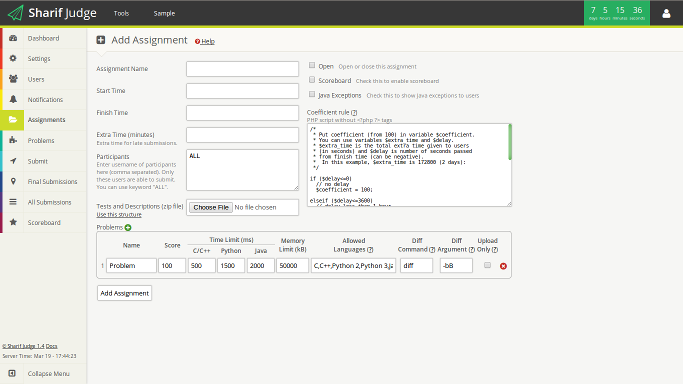
\includegraphics[scale=0.5]{add_assignment}  
	\caption[Tampilan Halaman \textit{Assignments}]{Tampilan Halaman \textit{Assignments}} 
	\label{fig:addass} 
\end{figure} 

Berikut beberapa pengaturan yang terdapat pada halaman \textit{Add Assignments}:
\begin{itemize}
	\item \textit{Assignment Name} \\
	Tugas akan ditampilkan dengan nama ini dalam daftar tugas.
	
	\item \textit{Start Time} \\
	\textit{Users} tidak dapat mengumpulkan tugas sebelum \textit{"Start Time"}. Gunakan format ini untuk \textit{start time}: \textit{MM/DD/YYYY HH:MM:SS}. Contoh: \textit{08/31/2013 12:00:00}
	
	\item \textit{Finish Time, Extra Time}\\
	\textit{Users} tidak dapat mengumpulkan tugas setelah \textit{Finish Time + Extra Time}. Tugas yang telat akan dikalikan dengan koefisien tertentu. Pengguna harus menulis \textit{script} PHP untuk menghitung koefisien pada bidang \textit{"Coefficient Rule"}. Gunakan format ini untuk \textit{finish time}: \textit{MM/DD/YYYY HH:MM:SS}. Contoh: \textit{08/31/2013 23:59:59}. Waktu ekstra harus dalam menit. Pengguna dapat menggunakan \textit{*}. Contoh \textit{120} (2 jam) atau \textit{48*60} (2 hari).
	
	\item \textit{Participants} \\
	Masukan \textit{username} dari partisipan disini. Gunakan tanda koma untuk memisah \textit{username} antar partisipan. Hanya \textit{users} ini yang dapat mengumpulkan tugas. Pengguna dapat menggunakan kata kunci \textit{ALL} untuk mengijinkan semua \textit{users} agar dapat mengumpulkan tugas. Contoh: \textit{admin, instructor1 , instructor2 ,student1  ,   student2,student3 , student4}.
	
	\item \textit{Open} \\
	Pengguna dapat membuka atau menutup tugas untuk \textit{students} menggunakan pilihan ini. Jika pengguna menutup tugas, \textit{non-student users} masih dapat mengumpulkan tugas.
	
	\item Scoreboard \\
	Pengguna dapat mengaktifkan atau mematikan papan nilai dengan menggunakan pilihan ini.
	
	\item \textit{Java Exceptions}
	Pengguna dapat mengaktifkan dan mematikan \textit{java exceptions} yang ditunjukan kepada \textit{students}. Perubahan pada pilihan ini tidak berdampak pada kode yang sebelumnya sudah dinilai. Nama \textit{exception} akan muncul jika \textit{tester/java\_exceptions\_list} berisikan nama tersebut. Jika pengguna mengaktifkan fitur ini, kode di bawah ini akan ditampilkan kepada \textit{students} saat \textit{exception} dilemparkan: \newpage
	\begin{lstlisting}[backgroundcolor = \color{lightgray}]
Test 1
ACCEPT
Test 2
Runtime Error (java.lang.ArrayIndexOutOfBoundsException)
Test 3
Runtime Error (java.lang.ArrayIndexOutOfBoundsException)
Test 4
ACCEPT
Test 5
ACCEPT
Test 6
ACCEPT
Test 7
ACCEPT
Test 8
Runtime Error (java.lang.ArrayIndexOutOfBoundsException)
Test 9
Runtime Error (java.lang.StackOverflowError)
Test 10
Runtime Error (java.lang.ArrayIndexOutOfBoundsException)
	\end{lstlisting}
	
	\item \textit{\textit{Coefficient Rule}} \\
	Pengguna dapat menulis \textit{script} PHP pada bagian ini. Pengguna harus memasukan koefisien (dari 100) pada variabel \textit{\$coefficient}. Pengguna dapat menggunakan variabel \textit{\$extra\_time} dan \textit{\$delay}. \textit{\$extra\_time} merupakan total waktu ekstra yang diberikan kepada \textit{users} dalam satuan detik dan \textit{\$delay} merupakan jumlah detik berlalu dari waktu selesai (bisa negatif). \textit{Script} PHP pada bagian ini tidak mengandung \textit{tags <?php , <? , ?>}. Berikut contoh \textit{\$extra\_time} 172800 (2 hari):
	\begin{lstlisting}[backgroundcolor = \color{lightgray}]
if ($delay<=0)
// no delay
$coefficient = 100;

elseif ($delay<=3600)
// delay less than 1 hour
$coefficient = ceil(100-((30*$delay)/3600));

elseif ($delay<=86400)
// delay more than 1 hour and less than 1 day
$coefficient = 70;

elseif (($delay-86400)<=3600)
// delay less than 1 hour in second day
$coefficient = ceil(70-((20*($delay-86400))/3600));

elseif (($delay-86400)<=86400)
// delay more than 1 hour in second day
$coefficient = 50;

elseif ($delay > $extra_time)
// too late
$coefficient = 0;
	\end{lstlisting}
	
	\item \textit{Time Limit} \\
	Pengguna dapat mengatur batas waktu untuk menjalankan kode dalam satuan milisekon. \textit{Python} dan \textit{Java} biasanya lebih lambat dari \textit{C/C++}.	Oleh karena itu mereka membutuhkan waktu yang lebih.
	
	\item \textit{Memory Limit} \\
	Pengguna dapat mengatur batas memori dalam satuan \textit{kilobyte}, namun penggunaan \textit{Memory Limit} tidak terlalu akurat.
	
	\item \textit{Allowed Languages} \\
	Pengguna dapat mengatur bahasa untuk setiap permasalahan (dipisahkan menggunakan koma). Bahasa yang tersedia seperti \textit{C, C++, Java, Python 2, Python 3, zip, PDF}. Pengguna dapat menggunakan \textit{zip} atau \textit{PDF} jika mengaktifkan pilihan \textit{Upload Only}. Contoh: \textit{C, C++ , zip} atau \textit{Python 2,Python 3} atau \textit{Java ,C}.
	
	\item \textit{Diff Command} \\
	\textit{Command} ini digunakan untuk membandingkan keluaran dengan keluaran yang benar. Secara \textit{default Sharif Judge} menggunakan \textit{diff}, namun pengguna dapat mengubah \textit{command} pada bagian ini.
	
	\item \textit{Diff Arguments} \\
	Pengguna dapat mengatur argumen dari\textit{Diff Command} disini. Untuk melihat daftar lengkap \textit{diff} argumen, pengguna dapat melihat \textit{man diff}. \textit{Sharif Judge} menambahkan dua pilihan baru yaitu \textit{ignore} dan \textit{identical}. \textit{Ignore} akan menghiraukan semua baris baru dan spasi. \textit{Identical} tidak akan menghiraukan apapun namun keluaran dari file yang dikumpulkan harus identik dengan keluaran \textit{test case} agar dapat diterima.
	
	\item \textit{Upload Only} \\
	Jika pengguna mengatur masalah sebagai \textit{Upload-Only}, maka \textit{Sharif Judge} tidak akan menilai tugas pada masalah tersebut. Pengguna dapat menggunakan \textit{zip} dan \textit{PDF} pada \textit{allowed languages} jika mengaktifkan pilihan ini.
\end{itemize}

\subsubsection{Contoh Tugas}

Berikut contoh tugas untuk mencoba \textit{Sharif Judge}. Menambah tugas ini dengan mengklik \textit{Add} di halaman \textit{Assignment}. Tugas dibagi menjadi 3 permasalahan:
\begin{enumerate}
	\item Masalah 1 (Penjumlahan) \\
	Program pengguna akan menerima masukan bilangan \textit{integer} n, kemudian menerima masukan lagi sebanyak n buah bilangan \textit{integer} dan menampilkan hasil penjumlahan dari n nomor tersebut. Untuk lebih jelas, perhatikan tabel~\ref{tab:tablesum}.
	
	\begin{table}[H] %atau h saja untuk "kira kira di sini"
		\centering 
		\caption{Masalah 1 (Penjumlahan)}
		\label{tab:tablesum}
		\begin{tabular}{cc}
			\toprule
			Sample Input & Sample Output\\
			
			\midrule
			\multicolumn{1}{l}{5} & \multirow{2}{*}{145}\\
			\multicolumn{1}{l}{54 78 0 4 9} & \\
			
			\bottomrule
			
		\end{tabular} 
	\end{table}
	
	\item Masalah 2 (\textit{Max}) \\
	Program pengguna akan menerima masukan bilangan \textit{integer} n, kemudian menerima masukan lagi sebanyak n buah bilangan \textit{integer} dan menampilkan hasil penjumlahan dari dua nilai tertinggi. Untuk lebih jelas, perhatikan tabel~\ref{tab:tablemax}.
	
	\begin{table}[H] %atau h saja untuk "kira kira di sini"
		\centering 
		\caption{Masalah 2 (\textit{Max})}
		\label{tab:tablemax}
		\begin{tabular}{cc}
			\toprule
			Sample Input & Sample Output\\
			
			\midrule
			\multicolumn{1}{l}{7} & \multirow{2}{*}{356}\\
			\multicolumn{1}{l}{162 173 159 164 181 158 175} & \\
			
			\bottomrule
			
		\end{tabular} 
	\end{table}
	
	\item Masalah 2 (\textit{Upload!}) \\
	Pengguna diharuskan mengunggah sebuah \textit{file} \textit{C} atau \textit{zip}. Masalah ini menggunakan pilihan \textit{"Upload Only} sehingga tidak akan dinilai oleh Sharif Judge.
\end{enumerate}

Pengguna dapat menemukan \textit{file zip} pada \textit{folder Assignments}. Perhatikan susunan pohon dari tugas ini:
\begin{lstlisting}[backgroundcolor = \color{lightgray}]
.
|-- p1
|   |-- in
|   |   |-- input1.txt
|   |   |-- input2.txt
|   |   |-- input3.txt
|   |   |-- input4.txt
|   |   |-- input5.txt
|   |   |-- input6.txt
|   |   |-- input7.txt
|   |   |-- input8.txt
|   |   |-- input9.txt
|   |   --- input10.txt
|   |-- out
|   |   --- output1.txt
|   |-- tester.cpp
|   --- desc.md
|-- p2
|   |-- in
|   |   |-- input1.txt
|   |   |-- input2.txt
|   |   |-- input3.txt
|   |   |-- input4.txt
|   |   |-- input5.txt
|   |   |-- input6.txt
|   |   |-- input7.txt
|   |   |-- input8.txt
|   |   |-- input9.txt
|   |   --- input10.txt
|   |-- out
|   |   |-- output1.txt
|   |   |-- output2.txt
|   |   |-- output3.txt
|   |   |-- output4.txt
|   |   |-- output5.txt
|   |   |-- output6.txt
|   |   |-- output7.txt
|   |   |-- output8.txt
|   |   |-- output9.txt
|   |   --- output10.txt
|   |-- desc.md
|   --- Problem2.pdf
|-- p3
|   --- desc.md
--- SampleAssignment.pdf
\end{lstlisting}
Masalah 1 menggunkan metode \textit{"Tester"} untuk mengecek keluaran sehingga memiliki \textit{file tester.cpp (Tester Script)}. Masalah 2 menggunakan metode \textit{Output Comparison} untuk mengecek keluaran sehingga memiliki dua \textit{folder} (\textit{in} dan \textit{out}) yang berisikan \textit{test case}. Masalah 3 merupakan masalah yang menggunakan pilihan \textit{Upload-Only}.

\subsubsection{Contoh Solusi}
Permasalahan diatas dapat diselesaikan menggunakan contoh solusi berikut ini:
\begin{itemize}
	\item Solusi Masalah 1 \\ 
	Menggunakan bahasa \textit{C}
	\begin{lstlisting}[backgroundcolor = \color{lightgray}]
#include<stdio.h>
int main(){
	int n;
	scanf("%d",&n);
	int i;
	int sum =0 ;
	int k;
	for(i=0 ; i<n ; i++){
		scanf("%d",&k);
		sum+=k;
	}
	printf("%d\n",sum);
		return 0;
}
	\end{lstlisting} 
	
	
	Menggunakan bahasa \textit{C++}
	\begin{lstlisting}[backgroundcolor = \color{lightgray}]
#include <iostream>
using namespace std;
int main(){
	int n, sum=0;
	cin >> n;
	for (int i=0 ; i<n ; i++){
		int a;
		cin >> a;
		sum += a;
	}
	cout << sum << endl;
	return 0;
}
	\end{lstlisting} 
	
	Menggunakan bahasa \textit{Java}
	\begin{lstlisting}[backgroundcolor = \color{lightgray}]
import java.util.Scanner;
class sum
{
	public static void main(String[] args)
	{ 
		Scanner sc = new Scanner(System.in);
		int n = sc.nextInt();
		int sum =0;
		for (int i=0 ; i<n ; i++)
		{
			int a = sc.nextInt();
			sum += a;
		}
		System.out.println(sum); 
	}
}
	\end{lstlisting}
	
	\item Solusi Masalah 2 \\ 
	Menggunakan bahasa \textit{C}
	\begin{lstlisting}[backgroundcolor = \color{lightgray}]
#include<stdio.h>
int main(){
	int n , m1=0, m2=0;
	scanf("%d",&n);
	for(;n--;){
		int k;
		scanf("%d",&k);
		if(k>=m1){
			m2=m1;
			m1=k;
		}
		else if(k>m2)
			m2=k;
	}
	printf("%d",m1+m2);
	return 0;
}
	\end{lstlisting}
	 
	
	Menggunakan bahasa \textit{C++}
	\begin{lstlisting}[backgroundcolor = \color{lightgray}]
#include<iostream>
using namespace std;
int main(){
	int n , m1=0, m2=0;
	cin >> n;
	for(;n--;){
		int k;
		cin >> k;
		if(k>=m1){
			m2=m1;
			m1=k;
		}
		else if(k>m2)
			m2=k;
		}
	cout << (m1+m2) << endl ;
	return 0;
}
	\end{lstlisting}
\end{itemize}

\subsection{Struktur Pengujian}

Pengguna harus menyediakan sebuah \textit{file zip} yang berisikan \textit{test cases} ketika menambahkan tugas. \textit{File zip} ini dapat berisikan folder-folder untuk setiap masalah. Pengguna harus memberikan nama pada folder sesuai aturan seperti \textit{p1, p2, p3, dst}. Tugas yang menggunakan pilihan \textit{Upload-Only} tidak membutuhkan \textit{folder}~\cite{mjnaderi:14:sharifjudgedoc}.

\subsubsection{Metode Pengecekan}
\textit{Sharif Judge} memiliki dua metode pengecekan untuk setiap permasalahan yaitu metode \textit{"Input/Output" Comparison} dan metode \textit{Tester}.
\begin{itemize}
	\item \textit{Metode Input/Output Comparison} \\
	Dengan metode ini, pengguna harus memasukan beberapa \textit{file input dan output} pada \textit{folder} masalah. \textit{Sharif Judge} akan memasukan nilai dari \textit{file input} ke kode \textit{users} dan membandingkan hasil keluaran dari kode \textit{users} dengan \textit{file output}. \textit{Input files} harus berada dalam folder \textit{"in"} dengan nama \textit{input1.text, input2.txt, dst}.\textit{Output files} harus berada dalam folder \textit{"out"} dengan nama \textit{output1.txt, output2.txt, dst}.
	
	\item \textit{Metode Tester} \\
	Dengan metode ini, pengguna harus menyediakan beberapa \textit{file input} dan sebuah \textit{file C++ (tester.cpp)} dan beberapa \textit{file output}. \textit{Sharif Judge} akan memasukan nilai dari \textit{file input} ke kode \textit{users} dan mengambil keluaran dari kode \textit{users}. \textit{tester.cpp} akan mengambil nilai dari \textit{file input, file output, }dan keluaran \textit{users}. Jika keluaran dari kode \textit{users} benar akan mengembalikan nilai 0, sebaliknya akan mengeluarkan nilai 1. Berikut contoh kode untuk menulis \textit{tester.cpp}:
	\begin{lstlisting}[backgroundcolor = \color{lightgray}]
/*
* tester.cpp
*/

#include <iostream>
#include <fstream>
#include <string>
using namespace std;
int main(int argc, char const *argv[])
{
	
	ifstream test_in(argv[1]);  /* Stream ini membaca 
	isi file input */
	ifstream test_out(argv[2]); /* Stream ini membaca 
	isi file output */
	ifstream user_out(argv[3]); /* Stream ini membaca 
	isi keluaran users */
	
	/* Kode Pengguna */
	/* Jika keluaran kode user benar, mengembalikan nilai 0, 
	sebaliknya mengembalikan 1 */
	
	...

}
	\end{lstlisting}
\end{itemize}

\subsubsection{Contoh \textit{File}}

Pengguna dapat menemukan contoh \textit{file} penguji pada \textit{folder Assignments}. Perhatikan susunan pohon dari \textit{file} tersebut:
\begin{lstlisting}[backgroundcolor = \color{lightgray}]
.
|-- p1
|   |-- in
|   |   |-- input1.txt
|   |   |-- input2.txt
|   |   |-- input3.txt
|   |   |-- input4.txt
|   |   |-- input5.txt
|   |   |-- input6.txt
|   |   |-- input7.txt
|   |   |-- input8.txt
|   |   |-- input9.txt
|   |   --- input10.txt
|   |-- out
|   |   --- output1.txt
|   --- tester.cpp
--- p2
	|-- in
	|   |-- input1.txt
	|   |-- input2.txt
	|   |-- input3.txt
	|   |-- input4.txt
	|   |-- input5.txt
	|   |-- input6.txt
	|   |-- input7.txt
	|   |-- input8.txt
	|   |-- input9.txt
	|   --- input10.txt
	--- out
		|-- output1.txt
		|-- output2.txt
		|-- output3.txt
		|-- output4.txt
		|-- output5.txt
		|-- output6.txt
		|-- output7.txt
		|-- output8.txt
		|-- output9.txt
		--- output10.txt
\end{lstlisting}

Masalah 1 menggunakan metode \textit{"Tester} untuk mengecek hasil keluaran, sehingga memiliki \textit{file tester.cpp}. Berikut isi dari \textit{file tester.cpp} untuk masalah 1:
\begin{lstlisting}[backgroundcolor = \color{lightgray}]
/*
* tester.cpp
*/

#include <iostream>
#include <fstream>
#include <string>
using namespace std;
int main(int argc, char const *argv[])
{
	
	ifstream test_in(argv[1]);  /* Stream ini membaca 
	isi file input */
	ifstream test_out(argv[2]); /* Stream ini membaca 
	isi file output */
	ifstream user_out(argv[3]); /* Stream ini membaca 
	isi keluaran users */
	
	/* Kode Pengguna */
	/* Jika keluaran kode user benar, mengembalikan nilai 0, 
	sebaliknya mengembalikan 1 */
	/* e.g.: Permasalahan: membaca n nomor dan keluarkan 
	hasil penjumlahannya: */
	
	int sum, user_output;
	user_out >> user_output;
	
	if ( test_out.good() ) // if test's output file exists
	{
		test_out >> sum;
	}
	else
	{
		int n, a;
		sum=0;
		test_in >> n;
		for (int i=0 ; i<n ; i++){
			test_in >> a;
			sum += a;
		}
	}
	
	if (sum == user_output)
		return 0;
	else
		return 1;

}
\end{lstlisting}


Masalah 2 menggunakan metode \textit{"Input/Output Comparison"} untuk mengecek hasil keluaran, sehingga memiliki dua folder \textit{in} dan \textit{out} yang berisikan \textit{test cases}. Masalah 3 menggunakan pilihan \textit{Upload-Only}, sehingga tidak memiliki folder apapun.

\subsection{Deteksi Kecurangan}
\textit{Sharif Judge} menggunakan \textit{Moss} untuk mendeteksi kode yang mirip. \textit{Moss (Measure Of Software Similarity)} merupakan sistem otomatis untuk menentukan kemiripan program. Pada saat ini, aplikasi utama \textit{Moss} telah digunakan untuk mendeteksi plagiarisme pada kelas \textit{programming}. Pengguna dapat mengirimkan kode final (yang dipilih oleh \textit{students} sebagai \textit{Final Submission}) ke \textit{server Moss} dengan satu klik~\cite{mjnaderi:14:sharifjudgedoc}.\\

Sebelum menggunakan \textit{Moss} ada beberapa hal yang harus diperhatikan yaitu:
\begin{itemize}
	\item Pengguna harus mendapatkan \textit{Moss user id} dan mengaturnya di \textit{Sharif Judge}. Untuk mendapatkan \textit{Moss user id}, pengguna harus terlebih dahulu daftar pada halaman \\ \textit{http://theory.stanford.edu/~aiken/moss/}. Pengguna akan mendapatkan sebuah \textit{email} yang berisikan \textit{script perl}. \textit{Moss user id} berada pada \textit{script} tersebut. \\
	Berikut potongan \textit{perl script} yang berisikan user id:

\begin{lstlisting}[backgroundcolor = \color{lightgray}]
...

$server = 'moss.stanford.edu';
$port = '7690';
$noreq = "Request not sent.";
$usage = "usage: moss [-x] [-l language] [-d] 
		  [-b basefile1] ... [-b basefilen] [-m #] 
		  [-c \"string\"] file1 file2 file3 ...";

#
# The userid is used to authenticate your queries to the server; 
  don't change it!
#
$userid=YOUR_MOSS_USER_ID;

#
# Process the command line options.  This is done in a non-standard
# way to allow multiple -b's.
#
$opt_l = "c";   # default language is c
$opt_m = 10;
$opt_d = 0;

...
}

\end{lstlisting}

\item Dapatkan \textit{user id} tersebut lalukan gunakan pada \textit{Sharif Judge} untuk mendetksi kecurangan. Pengguna dapat menyimpan \textit{user id} di Sharif Judge pada halaman \textit{Moss} dan \textit{Sharif Judge} akan menggunakan \textit{user id} tersebut di \textit{Moss perl script}.

\item \textit{Server} pengguna harus menginstal \textit{perl} untuk menggunakan \textit{Moss}.

\item Pengguna dianjurkan untuk mendetek kode yang mirip setelah waktu tugas berakhir, karena \textit{students} masih dapat mengubah \textit{Final Submissions} mereka sebelum waktu habis. Dengan cara tersebut \textit{Sharif Judge} dapat mengirimkan \textit{Final submissions student} ke \textit{Moss}.
\end{itemize}
